\documentclass[aspectratio=1610,onlymath]{beamer}
% \documentclass[aspectratio=1610,onlymath,handout]{beamer}

\input{macros-lecture}

\usepackage{setspace}
\usepackage{minted}

\defineTitle{2}{Äquivalenzen und Normalformen}{16. April 2026}

\begin{document}

\maketitle

\newcommand{\Aname}{Anna}
\newcommand{\Bname}{Barbara}
\newcommand{\Cname}{Chris}

\begin{frame}\frametitle{Rückblick: Aussagenlogik}

\emph{Syntax:}
\[ \Snterm{F}\to \Slang{P}\mid \Sterm{\neg}\Snterm{F}\mid\Sterm{(}\Snterm{F}\Sterm{\wedge}\Snterm{F}\Sterm{)} \mid\Sterm{(}\Snterm{F}\Sterm{\vee}\Snterm{F}\Sterm{)} \mid\Sterm{(}\Snterm{F}\Sterm{\to}\Snterm{F}\Sterm{)} \mid\Sterm{(}\Snterm{F}\Sterm{\leftrightarrow}\Snterm{F}\Sterm{)}
\]

\emph{Semantik:}
\begin{itemize}
\item Wertzuweisungen $w:\Slang{P}\to\{\mytrue,\myfalse\}$ zur Interpretation von Atomen
\item Erweiterung von Atomen auf Formeln:
\footnotesize
\narrowcentering{%
\begin{tabular}[t]{cc}
\rowcolor{lightblue!20}
$w(F)$ & $w(\neg F)$\\
\myfalse & \mytrue \\
\rowcolor{gray!10}
\mytrue & \myfalse \\
\end{tabular}}\medskip

\begin{tabular}{cccccc}
\rowcolor{lightblue!20}
$w(F)$ & $w(G)$ & $w(F\wedge G)$ & $w(F\vee G)$ & $w(F\to G)$ & $w(F\leftrightarrow G)$\\
\myfalse & \myfalse & \myfalse & \myfalse& \mytrue & \mytrue\\
\rowcolor{gray!10}
\mytrue & \myfalse & \myfalse & \mytrue& \myfalse & \myfalse\\
\myfalse & \mytrue & \myfalse & \mytrue& \mytrue & \myfalse\\
\rowcolor{gray!10}
\mytrue & \mytrue & \mytrue & \mytrue& \mytrue & \mytrue\\
\end{tabular}

\end{itemize}

\end{frame}

\begin{frame}\frametitle{Beispiel: Logelei}

\Aname{} behauptet: "`\Bname{} lügt!"'\hfill \visible<1->{$A\leftrightarrow \neg B$}
\bigskip

\Bname{} behauptet: "`\Cname{} lügt!"'\hfill \visible<1->{$B\leftrightarrow \neg C$}
\bigskip

\Cname{} behauptet: "`\Aname{} und \Bname{} lügen!"'\hfill \visible<1->{$C\leftrightarrow (\neg A\wedge \neg B)$}
\bigskip\bigskip

{\Large
\narrowcentering{\alert{Wer lügt?}}
}

\medskip
{\footnotesize\narrowcentering{(Und wie kann man das beweisen?)}}
% \bigskip

% 
% $A\leftrightarrow\neg B$
% $B\leftrightarrow\neg C$
% $C\leftrightarrow\neg A \wedge \neg B$

\end{frame}

\sectionSlide{Logische Konsequenzen}

\begin{frame}\frametitle{Logische Konsequenzen}

\defbox{Eine Wertzuweisung $w$ ist \redalert{Modell einer Formel $F$} wenn $w\models F$ (also wenn $w(F)=\mytrue$).
% Wir erweitern diese Notation auf (möglicherweise unendliche) Formelmengen: $w$ ist ein \redalert{Modell der Menge $\mathcal{F}$}
%  wenn $w\models F$ für alle $F\in\mathcal{F}$ gilt. In diesem Fall schreiben wir \redalert{$w\models\mathcal{F}$}.
% 
Ist $\mathcal{F}$ eine (möglicherweise unendliche) Menge von Formeln, dann ist $w$ ein \redalert{Modell der Menge $\mathcal{F}$}
 wenn $w\models F$ für alle $F\in\mathcal{F}$ gilt. In diesem Fall schreiben wir \redalert{$w\models\mathcal{F}$}.
}\pause

Die logischen Schlussfolgerungen aus einer Formel(menge) ergeben sich aus ihren Modellen:

\defbox{Sei $\mathcal{F}$ eine Menge von Formeln.
Eine Formel $G$ ist eine \redalert{logische Konsequenz} aus $\mathcal{F}$ wenn jedes Modell
von $\mathcal{F}$ auch ein Modell von $G$ ist.\\ In diesem Fall schreiben wir $\mathcal{F}\models G$.
}

\begin{enumerate}[$\leadsto$]
\item Die Formeln in $\mathcal{F}$ schränken die möglichen Interpretationen \ghost{ein:}\\
Je mehr Formeln wahr sein sollen,\\ desto weniger Freiheiten gibt es bei der Wahl der Modelle
\item $G$ ist eine logische Konsequenz wenn gilt:\\ Falls $\mathcal{F}$ wahr ist, dann ist auch $G$ garantiert wahr
% 
% Eine logische Konsequenz $G$ von $\mathcal{F}$ ist in jedem Fall (jedem Modell wahr in dem $\mathcal{F}$ wahr ist
\end{enumerate}

\end{frame}

\begin{frame}[t]\frametitle{Beispiel: Logelei}

\Aname{} behauptet: "`\Bname{} lügt!"'\hfill {$A\leftrightarrow \neg B$}\\[1ex]
\Bname{} behauptet: "`\Cname{} lügt!"'\hfill {$B\leftrightarrow \neg C$}\\[1ex]
\Cname{} behauptet: "`\Aname{} und \Bname{} lügen!"'\hfill {$C\leftrightarrow (\neg A\wedge \neg B)$}\\[2ex]

\begin{tabular}{c@{~ }c@{~ }cc@{\hspace{3mm}}c@{\hspace{3mm}}c}
\rowcolor{lightblue!20}
$w(A)$ & $w(B)$ & $w(C)$ & $w(A\leftrightarrow \neg B)$ & $w(B\leftrightarrow \neg C)$ & $w(C\leftrightarrow (\neg A\wedge \neg B))$\\
\myfalse & \myfalse & \myfalse & \myfalse& \myfalse & \myfalse\\
\rowcolor{gray!10}
\mytrue & \myfalse & \myfalse & \mytrue& \myfalse & \mytrue\\
\myfalse & \mytrue & \myfalse & \mytrue& \mytrue & \mytrue\\
\rowcolor{gray!10}
\mytrue & \mytrue & \myfalse & \myfalse& \mytrue & \mytrue\\
\myfalse & \myfalse & \mytrue & \myfalse& \mytrue & \mytrue\\
\rowcolor{gray!10}
\mytrue & \myfalse & \mytrue & \mytrue& \mytrue & \myfalse\\
\myfalse & \mytrue & \mytrue & \mytrue& \myfalse & \myfalse\\
\rowcolor{gray!10}
\mytrue & \mytrue & \mytrue & \myfalse& \myfalse & \myfalse\\
\end{tabular}

% {\Large
% \narrowcentering{\alert{Wer lügt?}}
% }
% 
% \medskip
% {\footnotesize\narrowcentering{(Und wie kann man das beweisen?)}}
% \bigskip


\end{frame}

\begin{frame}[t]\frametitle{Beispiel: Logelei (2)}

\Aname{} behauptet: "`\Bname{} lügt!"'\hfill {$A\leftrightarrow \neg B$}\\[1ex]
\Bname{} behauptet: "`\Cname{} lügt!"'\hfill {$B\leftrightarrow \neg C$}\\[1ex]
\Cname{} behauptet: "`\Aname{} und \Bname{} lügen!"'\hfill {$C\leftrightarrow (\neg A\wedge \neg B)$}\\[2ex]

\begin{tabular}{c@{~ }c@{~ }cc@{\hspace{3mm}}c@{\hspace{3mm}}c}
\rowcolor{lightblue!20}
$w(A)$ & $w(B)$ & $w(C)$ & $w(A\leftrightarrow \neg B)$ & $w(B\leftrightarrow \neg C)$ & $w(C\leftrightarrow (\neg A\wedge \neg B))$\\
% \myfalse & \myfalse & \myfalse & \myfalse& \myfalse & \myfalse\\
% \rowcolor{gray!10}
% \mytrue & \myfalse & \myfalse & \mytrue& \myfalse & \mytrue\\
\myfalse & \mytrue & \myfalse & \mytrue& \mytrue & \mytrue\\
% \rowcolor{gray!10}
% \mytrue & \mytrue & \myfalse & \myfalse& \mytrue & \mytrue\\
% \myfalse & \myfalse & \mytrue & \myfalse& \mytrue & \mytrue\\
% \rowcolor{gray!10}
% \mytrue & \myfalse & \mytrue & \mytrue& \mytrue & \myfalse\\
% \myfalse & \mytrue & \mytrue & \mytrue& \myfalse & \myfalse\\
% \rowcolor{gray!10}
% \mytrue & \mytrue & \mytrue & \myfalse& \myfalse & \myfalse\\
\end{tabular}

$\leadsto$ Genau ein Modell (bezüglich der relevanten Atome)
\pause\bigskip

\emph{Logische Konsequenzen:} Alle Formeln, die unter einer Wertzuweisung mit $w(A)=\myfalse$, $w(B)=\mytrue$ und $w(C)=\myfalse$ wahr sind, \ghost{z.B.:}
\begin{itemize}
\item $\neg A$ ("`\Aname{} lügt"')
\item $\neg C$ ("`\Cname{} lügt"')
\item $\neg A\wedge \neg C$ ("`\Aname{} und \Cname{} lügen"')
\item $B$ ("`\Bname{} sagt die Wahrheit"')
\item Aber auch: $D\vee \neg D$
\end{itemize}

% {\Large
% \narrowcentering{\alert{Wer lügt?}}
% }
% 
% \medskip
% {\footnotesize\narrowcentering{(Und wie kann man das beweisen?)}}
% \bigskip


\end{frame}


\begin{frame}\frametitle{Allgemeingültigkeit und Co.}

\defbox{Eine Formel $F$ ist:
\begin{itemize}
\item \redalert{unerfüllbar} (oder \alert{inkonsistent}), wenn sie keine Modelle hat
\item \redalert{erfüllbar} (oder \alert{konsistent}), wenn sie Modelle hat
\item \redalert{allgemeingültig} (oder eine \alert{Tautologie}), wenn alle Wertzuweisungen Modelle für die Formel sind
\item \redalert{widerlegbar}, wenn sie nicht allgemeingültig ist
\end{itemize}
Diese Begriffe kann man für Mengen von Formeln genauso definieren.
}

\examplebox{\emph{Beispiel:} 
\begin{itemize}
\item $p\wedge\neg p$ ist unerfüllbar (und widerlegbar)
\item $p\vee\neg p$ ist allgemeingültig (und erfüllbar)
\item $p\wedge q$ ist erfüllbar und widerlegbar
\end{itemize}}

\end{frame}

\begin{frame}\frametitle{Allgemeingültigkeit und Unerfüllbarkeit}

% Speziell Allgemeingültigkeit und Unerfüllbarkeit sind für logische Schlussfolgerung von Bedeutung:

\theobox{\emph{Satz:}
\begin{enumerate}[(1)]
\item Eine allgemeingültige Formel ist logische Konsequenz jeder anderen Formel(menge).
\item Eine unerfüllbare Formel(menge) hat jede andere Formel als logische Konsequenz.
\end{enumerate}}

\emph{Beweis:} Folgt direkt aus Definition von logischer Konsequenz. Für (2) ist es wichtig, dass eine Eigenschaft "`für alle Modelle"' gilt, wenn es keine Modelle gibt (sie gilt dann für "`alle null Modelle"'). \qed
\bigskip\pause

\anybox{purple}{
Der unerwartete(?) Effekt (2) ist im Deutschen sprichwörtlich:\medskip

\narrowcentering{"`Wenn das stimmt, dann bin ich der Kaiser von China!"'}\medskip

drückt aus, dass aus einer mutmaßlich falschen Annahme alles folgt, selbst wenn 
es offensichtlich unwahr ist.
}

\end{frame}


\begin{frame}\frametitle{Logische Schlussfolgerung}

\emph{Modelle:}\smallskip

$w\models F$ \alert{gdw.} $w(F)=\mytrue$ \alert{gdw.} "`$w$ ist Modell von $F$"' \alert{gdw.} "`$w$ erfüllt $F$"'
\bigskip

\emph{Logische Konsequenzen:}
\begin{itemize}
\item $\mathcal{F}\models G$ \alert{gdw.}
\item jedes Modell von $\mathcal{F}$ ist auch ein Modell von $G$ \alert{gdw.}
\item $G$ ist immer wahr wenn alle Formeln in $\mathcal{F}$ wahr sind
\end{itemize}\pause

\emph{Dualität von Modellen und Formeln:}
\begin{itemize}
\item Je mehr Formeln in $\mathcal{F}$
\item desto weniger Modelle erfüllen alle Formeln in $\mathcal{F}$
\item desto mehr Formeln sind in allen diesen Modellen wahr
\item desto mehr Konsequenzen hat $\mathcal{F}$
\end{itemize}
$\leadsto$ Aussagenlogik ist \redalert{monoton} (mehr Annahmen $\Rightarrow$ mehr Schlüsse)

\end{frame}

\sectionSlide{Modellierung in Aussagenlogik}

\begin{frame}\frametitle{Modellierungsbeispiel: Sudoku (1)}

Sudoku ist ein bekanntes Zahlenpuzzle.
\bigskip

\narrowcentering{
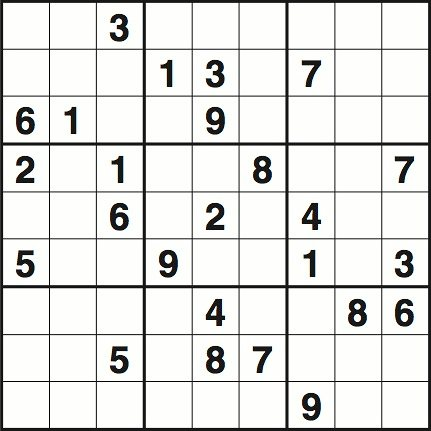
\includegraphics[height=4cm]{images/Sudoku}
}

Aufgabe: 
\begin{itemize}
\item Fülle jedes Feld mit einer Ziffer von $1$ bis $9$, so dass
\item Spalten, Zeilen und die fetten Teilquadrate jede Ziffer nur einmal enthalten
\end{itemize}

\end{frame}

\begin{frame}\frametitle{Modellierungsbeispiel: Sudoku (2)}

Wir können Sudoku aussagenlogisch modellieren:\pause

\begin{itemize}
\item \alert{Atome:} Für jede Ziffer $z\in\{1,\ldots,9\}$ und alle Koordinaten $i,j\in\{1,\ldots,9\}$ verwenden wir ein Atom $p_z[i,j]$ für die Aussage "`an Position $(i,j)$ steht die Ziffer $z$"'
\pause
\item \alert{Spielregeln} modellieren wir als logische Formeln:
\end{itemize}\vspace{-2.5ex}
\begin{align*}
\text{Für alle $i,j$:} & \quad p_1[i,j]\vee p_2[i,j]\vee\ldots\vee p_9[i,j] %& \quad\text{(mindestens eine Ziffer pro Feld)}
\\
\text{Für alle $i,j,z,z'$ mit $z\neq z'$:} & \quad p_z[i,j] \to \neg p_{z'}[i,j] %& \text{(höchstens eine Ziffer pro Feld)}
\\
\text{Für alle $i,i',j,z$ mit $i\neq i'$:} & \quad p_z[i,j] \to \neg p_z[i',j] %& \text{(höchstens eine Ziffer pro Feld)}
\\
\text{Für alle $i,j,j',z$ mit $j\neq j'$:} & \quad p_z[i,j] \to \neg p_z[i,j'] %& \text{(höchstens eine Ziffer pro Feld)}
\\
\text{Für alle $i,j,i',j',z$ mit $(i,j)\neq (i',j')$;}\\
\text{$(i,j)$, $(i',j')$  im gleichen Teilquadrat:} & \quad p_z[i,j] \to \neg p_z[i',j'] %& \text{(höchstens eine Ziffer pro Feld)}
\end{align*}\vspace{-4ex}\pause
\begin{itemize}
\item \alert{Vorgegebene Ziffern} werden als atomare Formeln dargestellt, z.B. $p_3[3,1]$ im vorigen Beispiel
\end{itemize}\pause
$\leadsto$ Modelle der Formelmenge entsprechen Lösungen des Sudoku

\end{frame}

\begin{frame}\frametitle{Logische Modellierung: Allgemeines Vorgehen}

Es ist oft nicht sofort ersichtlich, wie (oder ob) eine Problemstellung
gut in Aussagenlogik ausgedrückt werden kann.
\medskip

\anybox{strongyellow}{\emph{Allgemeines Vorgehen:}
\begin{enumerate}
\item \alert{Vokabular festlegen:} Welche Atome sollen verwendet werden, um eine Instanz der Frage und seiner Lösung darzustellen?
\item \alert{Bedingungen festlegen:} Welche aussagenlogischen Formeln müssen gelten, damit die Belegung der Atome eine korrekte Lösung des Problems kodiert?
\end{enumerate}}

\medskip
\begin{itemize}
\item Schritt 1 kann zu hunderten oder tausenden Atome führen (die ja jeweils nur ein \ghost{Bit)}\\ $\leadsto$ keine Angst vor großen Vokabularen
\item Schritt 2 kann je nach gewählter Kodierung direkter oder umständlicher sein\\ $\leadsto$ gegebenenfalls Kodierung aus Schritt 1 überdenken
\item Oft gut darstellbar: Aufgaben deren Lösung eine fest vorgegebene Größe hat und leicht überprüft werden kann (obwohl sie nicht leicht zu finden ist)\\
(Sudoku: Ja; nächster Zug im Schach: Nein (nicht einfach zu prüfen); Plan zum Lösen eines Sokoban-Puzzles: Nein (unbekannte, möglicherweise große \ghost{Schrittzahl))}
\end{itemize}

\end{frame}


\sectionSlide{Äquivalenzen}

\newcommand{\emphcell}[1]{\only<#1>{\cellcolor{strongyellow}}}

\begin{frame}\frametitle{Logische Äquivalenz}

Formeln sind äquivalent, wenn sie die gleiche Semantik haben:

\defbox{Zwei Formeln $F$ und $G$ sind \redalert{semantisch äquivalent}, in Symbolen \redalert{$F\equiv G$},
wenn sie genau die selben Modelle haben, d.h. wenn\\[1ex]

\narrowcentering{für alle Wertzuweisungen $w$ gilt: $w(F)=w(G)$}}\pause

\examplebox{Beispiel: $p\to q \equiv \neg p\vee q$, wie man mithilfe der Wahrheitswertetabelle zeigen kann (die Spalten der Formeln sind gleich):\smallskip

\narrowcentering{%
\begin{tabular}{cccccc}
\rowcolor{darkgreen!30}
$p$ & $q$ & $p\to q$ & $\neg p$ & $\neg p\vee q$ & ${}^*$\\
\myfalse & \myfalse & \emphcell{3-}{\mytrue} & \mytrue & \emphcell{3-}{\mytrue} \\
\mytrue & \myfalse & \emphcell{3-}{\myfalse} & \myfalse & \emphcell{3-}{\myfalse} \\
\myfalse & \mytrue & \emphcell{3-}{\mytrue} & \mytrue & \emphcell{3-}{\mytrue} \\
\mytrue & \mytrue & \emphcell{3-}{\mytrue} & \myfalse & \emphcell{3-}{\mytrue} \\
\end{tabular}}
}

{\footnotesize ${}^*$ Vereinfachung: Wir beschriften Tabellenspalten ab jetzt nur mit $F$ statt \ghost{$w(F)$.}}

\end{frame}

\begin{frame}\frametitle{Nützliche Eigenschaften von $\equiv$}

\theobox{\emph{Satz:} $\equiv$ ist eine Äquivalenzrelation, d.h. reflexiv, symmetrisch und transitiv.}

\emph{Beweis:} $\equiv$ ist definiert als die Gleichheit der Modellmengen. Die gesuchten Eigenschaften ergeben sich, da auch die Relation $=$ auf Mengen eine Äquivalenzrelation ist.\qed
\bigskip

Weitere Eigenschaften folgen direkt aus den Definitionen:\medskip

\theobox{\emph{Satz:}
\begin{itemize}
\item Alle Tautologien sind semantisch äquivalent
\item Alle unerfüllbaren Formeln sind semantisch äquivalent
\end{itemize}
}

% \emph{Beweis:} Offensichtlich sind die Modellmengen jeweils gleich.\qed

\theobox{\emph{Satz:} Semantische Äquivalenz entspricht wechselseitiger logischer Konsequenz:\\[1ex]
% 
\narrowcentering{ $F\equiv G$ \hspace{5mm}genau dann wenn\hspace{5mm} $F\models G$ und $G\models F$}
}

\end{frame}

\begin{frame}\frametitle{Nützliche Eigenschaften von $\equiv$}

% 
% \emph{Intuition:} Äquivalente Formeln sind untereinander austauschbar, da sie sich logisch immer gleich verhalten
% \bigskip


\theobox{\emph{Satz (Ersetzungstheorem):} Sei $F$ eine Formel mit einer Teilformel $G$. 
Wenn $G\equiv G'$ und wenn $F'$ aus $F$ gebildet werden kann, indem man ein beliebiges Vorkommen von $G$ in $F$ durch $G'$ ersetzt, dann gilt auch $F\equiv F'$.}\pause

\emph{Beweisskizze${}^*$:} Aus $G\equiv G'$ folgt, dass $w\models G$ gdw. $w\models G'$ für beliebige Wertzuweisungen $w$ gilt.
% Gemäß der rekursiven Definition von $\models$ hängt $w\models H$ nur davon ab, welche der direkten Unterformeln von
% $H$ durch $w$ erfüllt sind.
In der rekursiven Definition von $\models$ erfüllt daher die Teilformel $G$ genau die selben Bedingungen wie $G'$, so
dass sich auch für $F$ und $F'$ der selbe Wert ergibt.\qed
\bigskip

Dieser Satz ist ein Sonderfall der allgemeingültigen und intuitiven Tatsache, dass der Wert von rekursiv definierten Funktionen gleich bleibt, wenn man die syntaktische Definition einer Teilberechnung durch eine andere ersetzt, die stets den gleichen Wert liefert.
\bigskip

\setstretch{0.9}

{\tiny ${}^*$ Streng genommen folgt aus der Definition von $\models$ zunächst nur, dass die Ersetzung einer direkten Unterformel
Äquivalenz erhält. Zum Beispiel folgt $G\wedge H\equiv G'\wedge H$ aus $G\equiv G'$. Um zu zeigen, dass auch Ersetzungen in beliebiger Tiefe Äquivalenz erhalten, ist noch ein induktives Argument nötig, welches die Äquivalenz im Formelbaum "`nach oben"' propagiert. Aus $G\wedge H\equiv G'\wedge H$ folgt z.B. $(G\wedge H)\vee J\equiv (G'\wedge H)\vee J$ usw. usf.
}

\end{frame}

\begin{frame}\frametitle{Junktoren äquivalent ausdrücken}

Viele Junktoren können durch andere ausgedrückt werden:
% 
\begin{align*}
F\to G & \equiv \neg F\vee G \equiv \neg(F\wedge\neg G) \\
F\leftrightarrow G & \equiv (F\to G)\wedge(G\to F)\equiv (F\wedge G)\vee(\neg F\wedge \neg G) \\
F\wedge G & \equiv \neg(\neg F\vee\neg G) \quad \text{\textcolor{devilscss}{(De Morgansches Gesetz)}} \\
F\vee G & \equiv \neg(\neg F\wedge\neg G) \quad \text{\textcolor{devilscss}{(De Morgansches Gesetz)}}
\end{align*}\pause
%
Weitere Junktoren können mithilfe äquivalenter Formeln definiert werden:
% 
\begin{align*}
F\uparrow G & \equiv \neg (F\wedge G) \equiv \neg F\vee \neg G & \text{\textcolor{devilscss}{(NAND)}}\\
F\downarrow G & \equiv \neg (F\vee G) \equiv \neg F\wedge \neg G & \text{\textcolor{devilscss}{(NOR)}}\\
\top & \equiv \neg p\vee p \equiv p\to p & \text{\textcolor{devilscss}{(Wahrheit; $p\in\Slang{P}$ beliebig)}} \\
\bot & \equiv \neg p\wedge p & \text{\textcolor{devilscss}{(Falschheit; $p\in\Slang{P}$ beliebig)}}
\end{align*}\vspace{-4ex}

Wir werden insbesondere $\top$ und $\bot$ manchmal verwenden.

\end{frame}

\begin{frame}\frametitle{Junktoren äquivalent ausdrücken (2)}

% Mit dem Ersetzungstheorem folgt nun leicht:\medskip

\theobox{\emph{Satz:} Sei $F$ eine beliebige aussagenlogische Formel.
\begin{itemize}
\item Es gibt eine zu $F$ äquivalente Formel, die nur die Junktoren $\wedge$ und $\neg$ enthält.
\item Es gibt eine zu $F$ äquivalente Formel, die nur die Junktoren $\vee$ und $\neg$ enthält.
\end{itemize}}\pause

\emph{Beweis:} Für den ersten Fall ersetzen wir iterativ Teilformeln, die nicht die gewünschte Form haben, gemäß den folgenden Regeln:
\begin{align*}
(G\vee H) &\qquad\mapsto\qquad \neg(\neg G\wedge\neg H)\\
(G\to H) &\qquad\mapsto\qquad\neg (G\wedge\neg H)\\
(G\leftrightarrow H) &\qquad\mapsto\qquad (\neg (G\wedge\neg H)\wedge\neg (H\wedge\neg G))
\end{align*}
Jede Ersetzung führt zu einer äquivalenten Formel (Ersetzungstheorem), der Algorithmus terminiert (jeder Junktor wird höchstens einmal ersetzt) und das Ergebnis hat die gewünschte Form.
% 
Der zweite Fall ist analog.
\qed

\end{frame}

\begin{frame}\frametitle{Nützliche Äquivalenzen (1)}

\begin{align*}
\begin{split}
F\wedge G & \equiv G\wedge F\\
F\vee G & \equiv G\vee F
\end{split}
		& \text{\textcolor{devilscss}{Kommutativität}} \\[1ex]
%
\begin{split}
(F\wedge G)\wedge H & \equiv F\wedge (G\wedge H)\\
(F\vee G)\vee H & \equiv F\vee (G\vee H)
\end{split}
		& \text{\textcolor{devilscss}{Assoziativität}} \\[1ex]
%
\begin{split}
F\wedge (G\vee H) & \equiv (F\wedge G) \vee (F\wedge H)\\
F\vee (G\wedge H) & \equiv (F\vee G)\wedge (F\vee H)
\end{split}
		& \text{\textcolor{devilscss}{Distributivität}} \\[1ex]
%
\begin{split}
F\wedge F & \equiv F\\
F\vee F & \equiv F
\end{split}
		& \text{\textcolor{devilscss}{Idempotenz}} \\[1ex]
%
\begin{split}
F\wedge (F\vee G) & \equiv F\\
F\vee (F\wedge G) & \equiv F
\end{split}
		& \text{\textcolor{devilscss}{Absorption}}
\end{align*}

\end{frame}

\begin{frame}\frametitle{Nützliche Äquivalenzen (2)}

\begin{align*}
\neg\neg F &\equiv F
		& \text{\textcolor{devilscss}{doppelte Negation}}\\[1ex]
%
\begin{split}
\neg(F\wedge G) & \equiv (\neg F\vee \neg G)\\
\neg(F\vee G) & \equiv (\neg F\wedge \neg G)
\end{split}
		& \text{\textcolor{devilscss}{De Morgansche Gesetze}} \\[1ex]
%
\begin{split}
F\wedge \top & \equiv F\\
F\vee \top & \equiv \top
\end{split}
		& \text{\textcolor{devilscss}{Gesetze mit $\top$}}\\[1ex]
%
\begin{split}
F\wedge \bot & \equiv \bot\\
F\vee \bot & \equiv F
\end{split}
		& \text{\textcolor{devilscss}{Gesetze mit $\bot$}}\\[1ex]
%
\begin{split}
\neg\top & \equiv \bot\\
\neg\bot & \equiv \top
\end{split}
		& 
\end{align*}

Alle diese Äquivalenzen können leicht mit Wahrheitswertetabellen überprüft werden.

\end{frame}

\begin{frame}\frametitle{Äquivalente Mengen von Formeln}

Die Definition von Äquivalenz ist leicht auf Formelmengen erweiterbar:\medskip

\defbox{Zwei Formelmengen $\mathcal{F}$ und $\mathcal{G}$ sind äquivalent, in Symbolen $\mathcal{F}\equiv\mathcal{G}$, wenn sie die selben Modelle haben.}\medskip\pause

Formelmengen verallgemeinern die Konjunktion, denn es gilt:\\[0.5ex]
%
\narrowcentering{
$ \{F_1,\ldots, F_n\}\equiv \{ F_1\wedge\ldots\wedge F_n\}$}\\[1ex]
%
\emph{Vereinfachung:} Dank Assoziativität verzichten wir ab jetzt in Formeln wie $(((F_1\wedge F_2)\wedge F_3)\wedge F_4)$
auf Klammern (ebenso für $\vee$).
\bigskip

Allerdings dürfen Formelmengen auch unendlich sein (Konjunktionen dagegen nicht).

\end{frame}

\begin{frame}\frametitle{$\models$ entspricht $\to$ und $\equiv$ entspricht $\leftrightarrow$}

\theobox{\emph{Satz (Deduktionstheorem):} Für jede Formelmenge $\mathcal{F}$ und Formeln $G$ und $H$ gilt $\mathcal{F}\models G\to H$ genau dann wenn $\mathcal{F}\cup\{G\}\models H$.}\pause

\emph{Beweis:} Einfache Anwendung der Definitionen.
($\Rightarrow$) Wenn jedes Modell von $\mathcal{F}$ die Formel $G\to H$ erfüllt, 
dann muss jedes dieser Modelle, welches zudem $G$ erfüllt, $H$ erfüllen.  ($\Leftarrow$) Wenn jedes Modell von $\mathcal{F}$, welches zudem $G$ erfüllt, auch $H$ erfüllt, dann muss jedes Modell von $\mathcal{F}$ auch $G\to H$ erfüllen.\qed\medskip\pause

\anybox{purple}{\emph{Notation:}
Wir schreiben $\models F$ statt $\emptyset\models F$ um auszudrücken, dass $F$ allgemeingültig ist.}

\theobox{\emph{Satz:} $F\equiv G$ genau dann wenn $\models F\leftrightarrow G$.}\pause

\emph{Beweis:} $F\equiv G$ \alert{gdw.} $F\models G$ und $G\models F$ \alert{gdw.} $\models F\to G$ und $\models G\to F$ (wegen Deduktionstheorem) \alert{gdw.} $\models F\leftrightarrow G$. \qed

\end{frame}

\begin{frame}\frametitle{Curry}

Mit Deduktionstheorem und dem Bezug von Formelmengen und Konjunktionen erhält man ein weiteres interessantes
Ergebnis:\medskip

\narrowcentering{%
\begin{tabular}{@{}r@{~~}l@{~~}l@{}}
$\models (F\wedge G)\to H$ & gdw. $\{F\wedge G\}\models H$ & gdw. $\{F,G\}\models H$ \\
	& gdw. $\{F\}\models G\to H$ & gdw. $\models F\to (G\to H)$\\[1ex]
\end{tabular}}\medskip\pause

Tatsächlich gilt allgemein:
% 
\[ (F\wedge G)\to H\equiv F\to (G\to H)\]
% 
Die Ersetzung von $(F\wedge G)\to H$ durch $F\to (G\to H)$ wird \alert{Currying} (im Deutschen manchmal
auch: \alert{Schönfinkeln}) genannt\\
$\leadsto$ vgl. \redalert{funktionale Programmierung}

\end{frame}

\sectionSlide{Aussagenlogisch Schließen in der Praxis}

\begin{frame}\frametitle{SAT Solver}

Programme zum aussagenlogischen Schließen heißen \alert{SAT Solver}.
\begin{itemize}
\item Hochoptimierte Systeme treten auf der jährlichen SAT-Competition gegeneinander an (\url{https://satcompetition.github.io/})
\item Praxissysteme sind teils weniger extrem optimiert aber anwendungsfreundlicher oder vielseitiger
\item Alle relevanten Programmiersprachen sollten geeignete Bibliotheken anbieten, zumeist frei und open source
\item Oft mit weiteren Features (nicht-boolesche Datentypen, weiche Optimierungskriterien, bestimmte prädikatenlogische Features, usw.)
\end{itemize}
\redalert{$\leadsto$ wir werden mit Z3 in Python arbeiten}

\end{frame}

\newcommand{\terminalbox}[1]{\begin{tikzpicture}%
\node [draw=black!50, fill=black!80, very thick, rectangle, rounded corners, inner sep=10pt, inner ysep=10pt, align=left, text width=0.8\linewidth] (box){%
\textcolor{white}{\texttt{#1}}
};%
\end{tikzpicture}}

\begin{frame}[fragile]\frametitle{Der SMT-Solver Z3}

\alert{Z3 ist ein leistungsfähiger Theorembeweiser}
\begin{itemize}
\item Typ SMT-Solver (insbesondere vollständig \& korrekt für Aussagenlogik)
\item Ursprüngliches Anwendungsgebiet Softwareverifikation; inzwischen vielfältig eingesetzt
\item Frei und OSS (MIT-Lizenz), entwickelt von Microsoft Research seit 2012
\item C++, viele Sprachbindungen (Python, JavaScript, C, Rust, Java, \ldots) sowie Unterstützung des Austauschformats SMTLIB2\\[1ex]
\terminalbox{pip~install~z3-solver}
\end{itemize}
\medskip

Dokumentation: \url{https://microsoft.github.io/z3guide/}\\($\to$Programming Z3$\to$Python)

\end{frame}

\begin{frame}[fragile]\frametitle{Z3 in Python}

\begin{tikzpicture}%
\node [draw=black!50, fill=white, very thick, rectangle, rounded corners, inner sep=10pt, inner ysep=10pt, align=left, text width=0.8\linewidth] (box){%
\vspace{-2ex}
\begin{minted}{python}
from z3 import *

p,q,r = Bools('p q r')

s = Solver()
s.add(And(p, Or(Not(q), r)))

print(s.check())
print(s.model())
\end{minted}
};%
\end{tikzpicture}\medskip\pause

\terminalbox{sat\newline
[p = True, q = False, r = False]}


\end{frame}



\begin{frame}\frametitle{Zusammenfassung und Ausblick}

Die Modelle einer Formel(menge) definieren ihre \redalert{logischen Konsequenzen}
(="`alles, was in diesen Fällen noch gilt"')\bigskip

In der Aussagenlogik gelten viele \redalert{nützliche Äquivalenzen} die man für Umformungen ausnutzen kann
\bigskip

Es gibt viele freie Softwarepakete zum aussagenlogischen Schließen, zum Beispiel \redalert{Z3}
\bigskip

\anybox{yellow}{
Offene Fragen:
\begin{itemize}
\item Wie funktioniert logisches Schließen ohne Wahrheitswertetabellen?
\item Wie (in)effizient ist logisches Schließen?
\item Was hat das mit Komplexität zu tun?
\end{itemize}
}

\end{frame}


\end{document}
